\section{Research Design}
\label{sec:researchdesign}

\todo[inline,color=cyan,author=Pedro]{Describe research design}
\todo[inline,color=cyan,author=Pedro]{Improve RQ descriptions}

\begin{description}
\item[RQ1:] \textit{Which API is easier to learn and use according to the student perceptions?}
\item[RQ2:] \textit{Which API is better to improve the performance according to the student perceptions?}
\end{description}

\subsection{Students' Background}

\todo[inline,color=cyan,author=Pedro]{Describe students' background}

\begin{figure}[htpb]
    \centering
    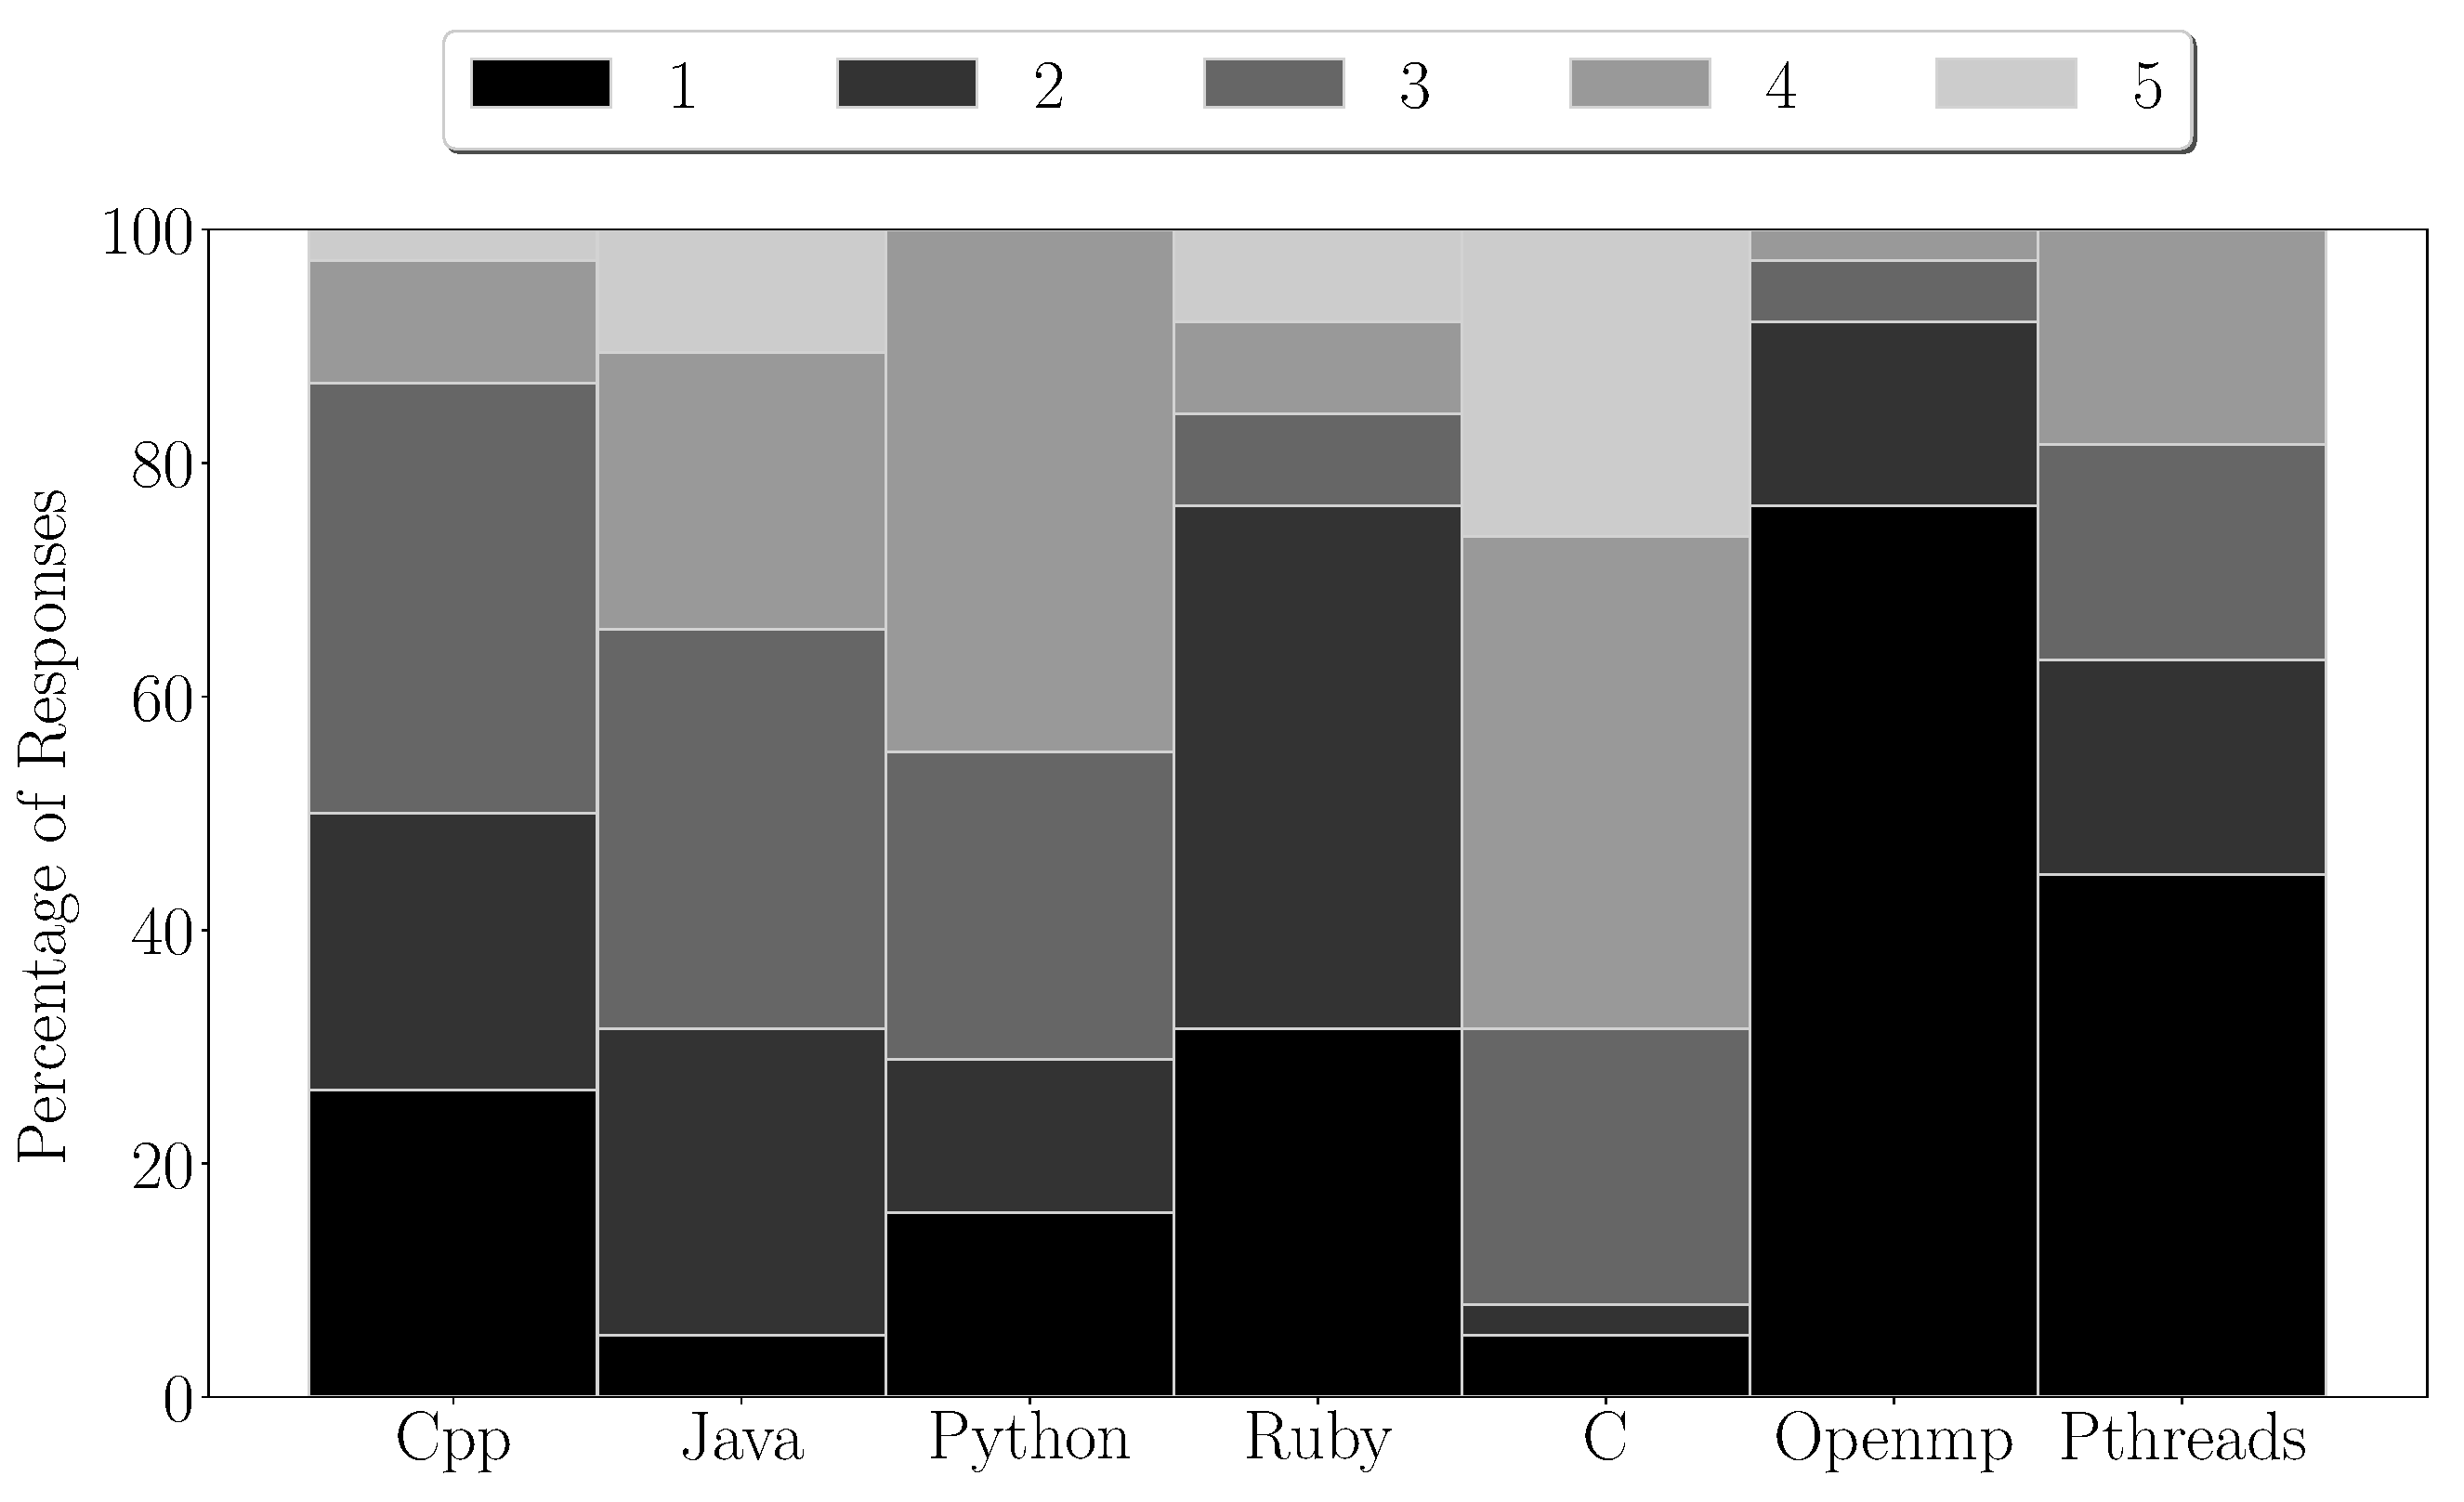
\includegraphics[width=0.85\columnwidth]{background_questions}
    \caption{Student mean knowledge \textit{before} the assignment}
    \label{fig:background}
\end{figure}

\begin{table}[htpb]
    \centering
    \begin{tabular}{@{}p{0.9\columnwidth}p{0.08\columnwidth}@{}}
        \toprule
        \multicolumn{1}{c}{\scriptsize{Have you$\dots$}} & \textnumero \\ \midrule
        \scriptsize{Had contact with parallel and distributed concepts before?} & $(1)$ \\
        \scriptsize{Had contat with the APIs before?} & $(2)$ \\
        \scriptsize{Learned from the OpenMP class?} & $(3)$ \\
        \scriptsize{Learned from the Pthreads class?} & $(4)$ \\ \bottomrule
    \end{tabular}
    \caption{Questions for Figure \ref{fig:classes}}
    \label{tab:classes}
\end{table}

\begin{figure}[htpb]
    \centering
    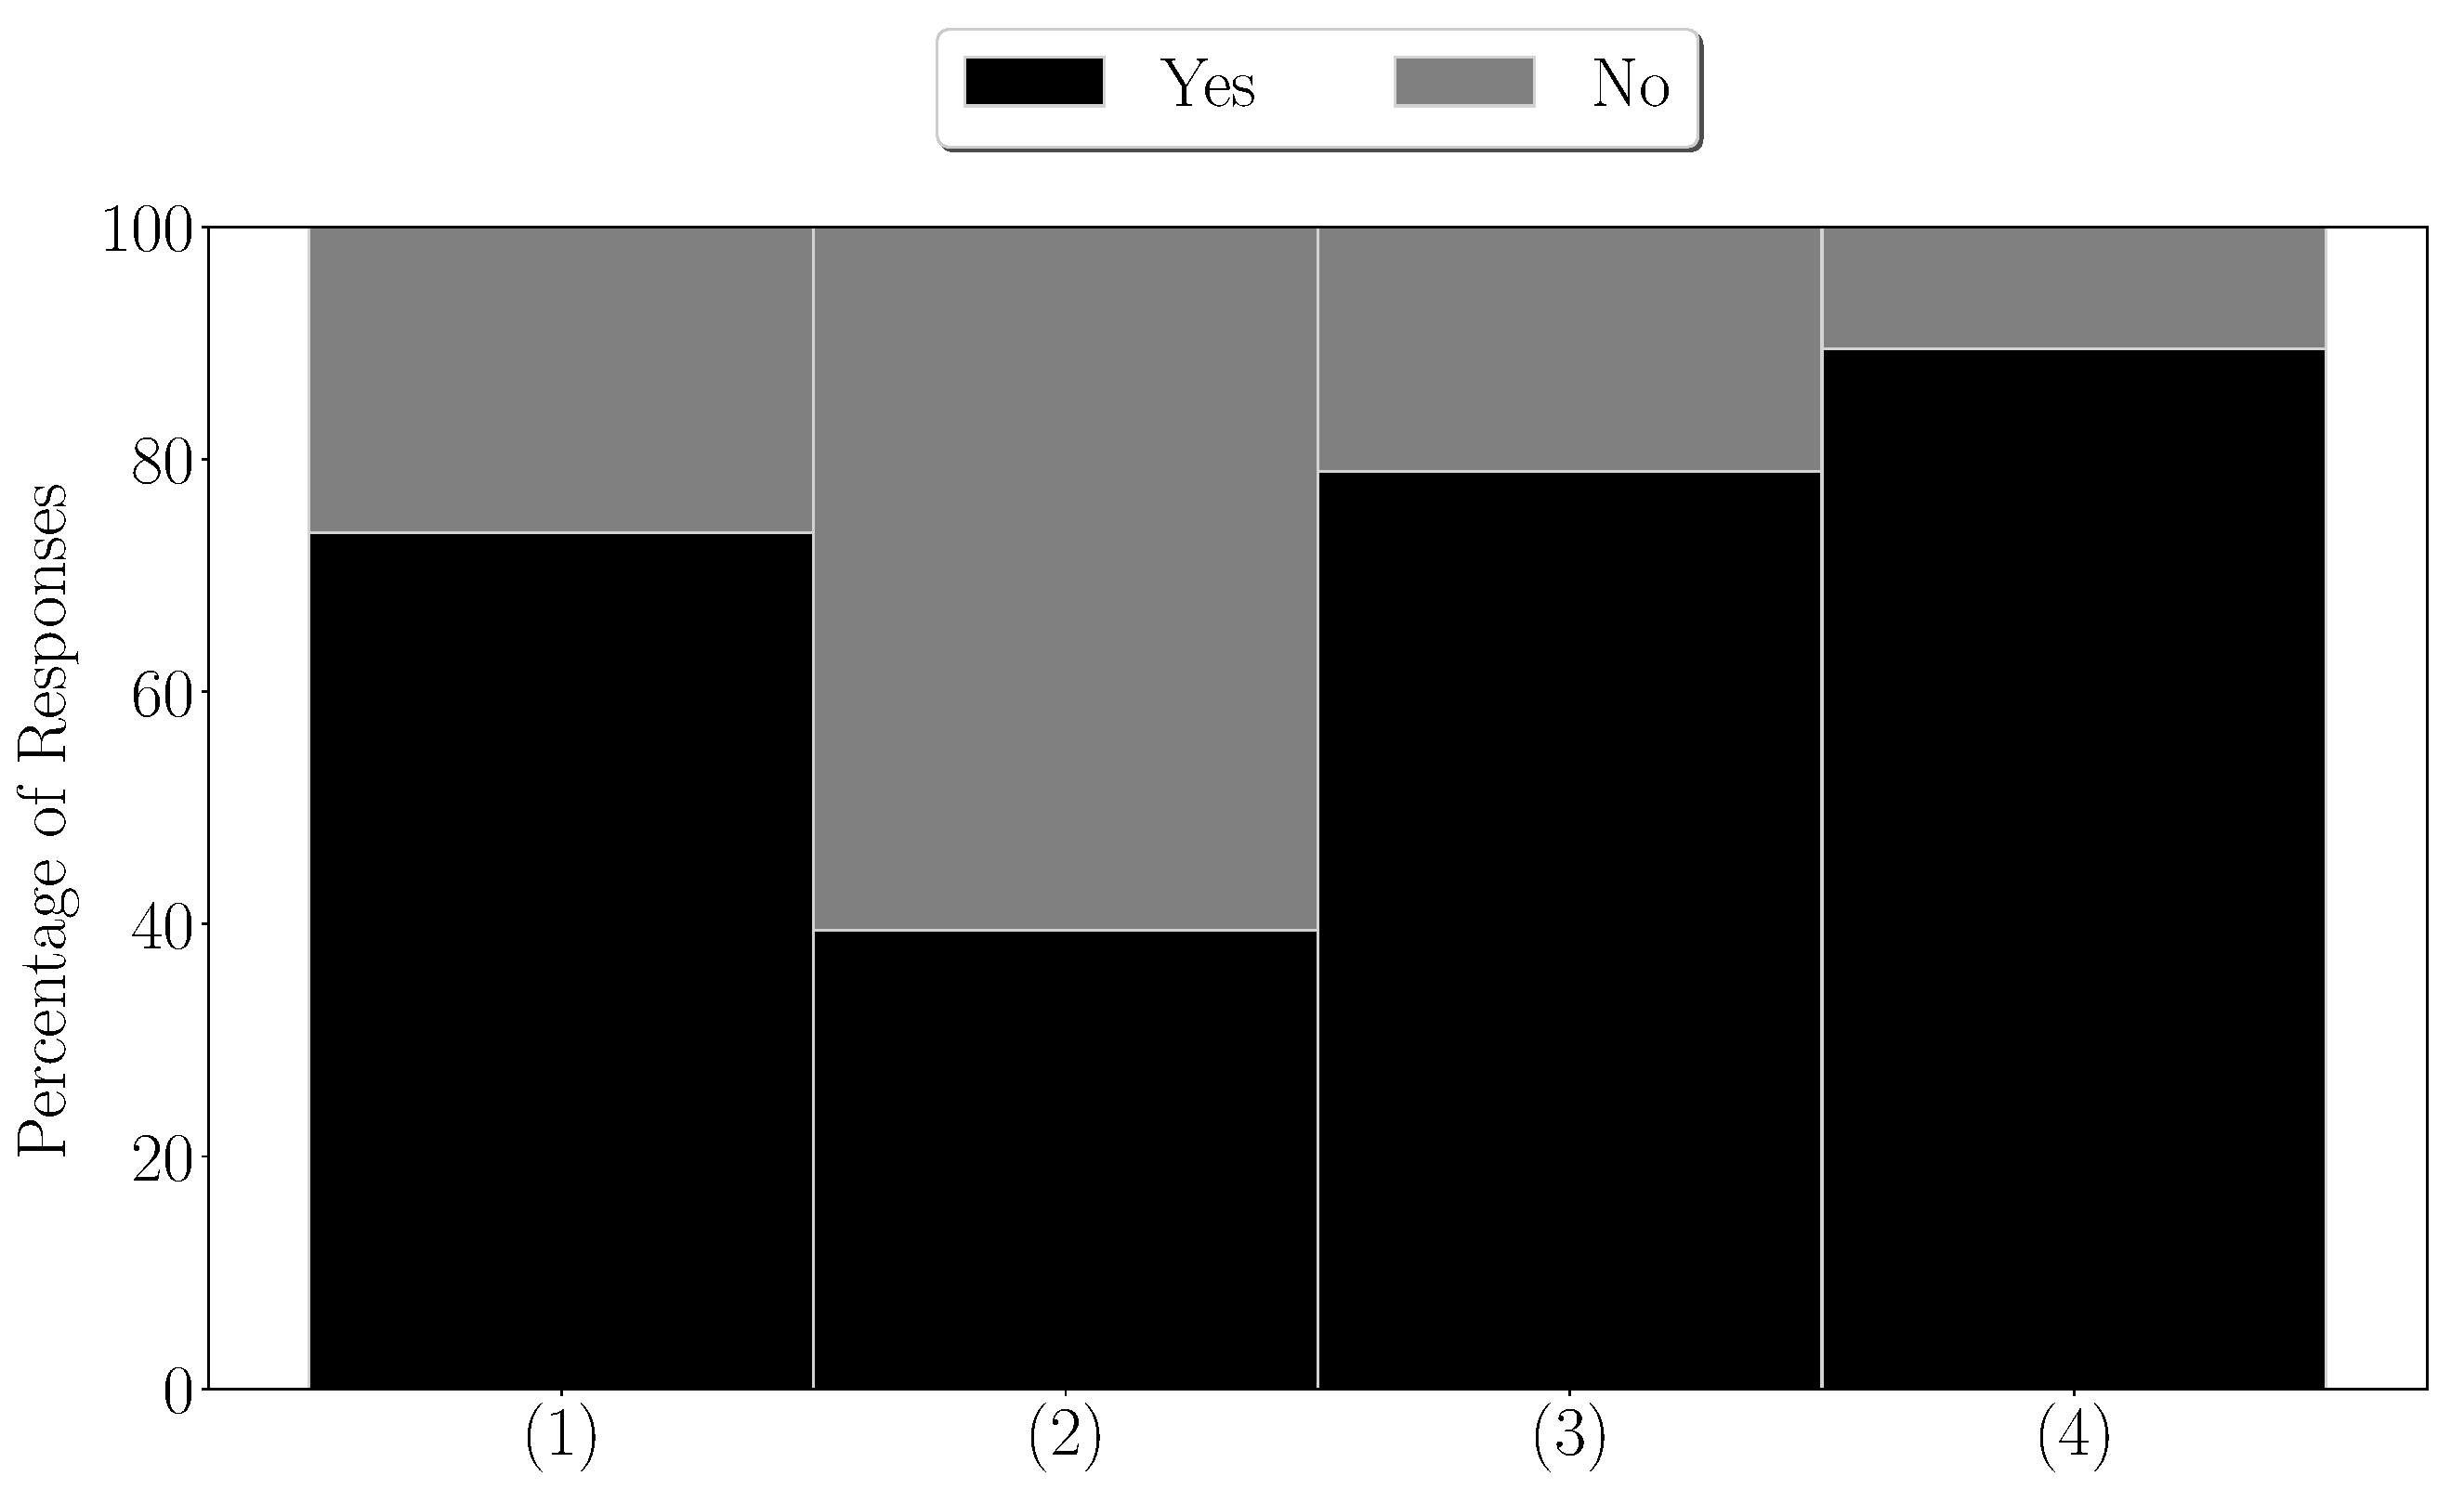
\includegraphics[width=0.85\columnwidth]{classes_questions}
    \caption{Student API knowledge \textit{before} the assignment and their relation to classes}
    \label{fig:classes}
\end{figure}


